\chapter{Future Works and Conclusion}\label{chap:conclusion}
Certain measurable quantities are valued because of the information they reveal about the geometry of the Fermi surface. Additionally, these quantities are attractive because they depend only on universal constants, experimentally controlled variables, and information about the electronic band structure which is entirely determined by the shape of the Fermi surface \cite{Ashcroft_SolidStatePhysics1978}. These measurable quantities commonly arise in the presence of a strong magnetic field and low temperature system. Determining the Fermi surface geometry provides insight into the transport and scattering properties of the material.

\section{Integer Quantum Hall Effects}\label{sec:IQHE}
In a \ac{2DES} there are a number of interesting phenomena that occurs at low temperatures in the presence of strong magnetic fields. One such effect is the \ac{IQHE}. The \acs{IQHE} was discovered in 1980 by Klitzing \emph{et al.} \cite{Klitzing_PhysRevLett1980}. They showed that under a quantum regime of temperature and magnetic field there is a quantization of the Hall resistance, which deviates from its linearity in the magnetic field seen in the classical Hall effect, displaying plateaus at particular values of the magnetic field where the Hall resistance is given purely in terms of universal constants. In addition, the plateaus observed in the Hall resistance are accompanied by a vanishing longitudinal resistance \cite{Klitzing_PhysRevLett1980,Ando_RevModPhys1982,Goerbig_2009,Hook_Solid1991}.\\ \\

%\subsection{Theoretical Background}\label{subsec:IQHE_theory}
\noindent In order to fully mathematically describe the theory behind the \acs{IQHE} one must first introduce the concept of Landau levels. Here we assume a quantum regime in which there is a low temperature and high magnetic field such that $\hbar\omega\gg k_B T$. The Hamiltonian of a particle in a uniform magnetic field is given by 
\begin{equation}\label{eq:particle_in_b_field}
\hat{H} = \frac{1}{2m}\left(\hat{p}_x+eBy/c\right)^2 + \frac{\hat{p}_y^2}{2m} + \frac{\hat{p}_z}{2m} - \left(\mu/s\right)\hat{s}_z B,
\end{equation}
where $\hat{p}_i$ is the momentum operator in the specified coordinate direction, $B$ is the magnetic field, $e$ is the charge of an electron, $\left(\mu/s\right)\hat{s}_z$ is the intrinsic magnetic moment operator \cite{Landau_Quantum1965}. It is worth noting that the vector potential chosen in eq.~\ref{eq:particle_in_b_field} is known as the Landau gauge, $\vec{A} = \left(-By, 0, 0\right)$, which implies the magnetic field $B$ is directed in the positive $z$-direction \cite{Sakurai_Quantum1994,Landau_Diagmagnetismus1930}. In this case the eigenfunctions of the Hamiltonian must take the form,
\begin{equation}\label{eq:psi_b_field}
\psi\left(\vec{r}\right) = e^{\left(i/\hbar\right)\left(p_x x+p_z z\right)}\chi\left(y\right),
\end{equation} 
where $\chi\left(y\right)$ is defined by solutions to  
\begin{equation}\label{eq:b_field_schrodinger}
	\frac{\partial^2 \chi}{\partial y^2} + \frac{2m}{\hbar^2}\left[E +\left(\mu/s\right)\sigma B - \frac{p_z^2}{2m}-\frac{1}{2}m\left(\frac{e B}{mc}\right)^2\left(y-y_0\right)^2\right]\chi = 0,
\end{equation}
where $y_0 =-c p_x/e B$ and $\omega = \abs{e}B/m c$. Additionally, since the Hamiltonian does not explicitly depend on $x$ and $z$ this implies that both the $x$ and $z$ components of the generalized momentum are conserved. Eq.~\ref{eq:b_field_schrodinger} is formally identical to that of the linear oscillator, thus the expression for the energy levels of a particle in a uniform magnetic field is 
\begin{equation}\label{eq:landau_levels_3D}
	E = \left(n+\frac{1}{2}\right)\frac{\abs{e}\hbar B}{mc} + \frac{p_z^2}{2m} - \left(\mu/s\right)\sigma B,
\end{equation}
where $n$ is any integer \cite{Landau_Quantum1965}. These quantum numbers $n$ specify states known as Landau levels. For the case in which the motion of particles in restricted to a rectangular geometry of $L_x \times L_y$, also let $p_z=0$ as the motion of particles is restricted in this case to only the $x-y$ plane. In this case the energy of each Landau level is given by 
\begin{equation}\label{eq:landau_levels_2D}
	E = \left(n+\frac{1}{2}\right)\frac{\abs{e}\hbar B}{mc} - \left(\mu/s\right)\sigma B.
\end{equation}
Due to the restriction that $\hbar\omega \gg k_B T$, thermal excitations can be neglected because the interval between Landau levels is much greater than thermal excitation energy. As a result, the probability that electrons will be thermally excited to higher energy levels can be neglected. In order to fill higher energy levels the density of states must be increased. When the Landau level is fully occupied from the lowest to the $i\mathrm{th}$ energy level the transverse resistivity becomes
\begin{equation}\label{eq:rho_xy}
	\rho_{xy} = \frac{h}{i e^2},
\end{equation}
where $i$ is any integer corresponding to a specific filled Landau level, $e$ is the charge of an electron, and $h$ is Planck`s constant \cite{Klitzing_PhysRevLett1980,Goerbig_2009}. Eq.~\ref{eq:rho_xy} shows that at critical values of the field, the Hall resistivity (or conductivity) is quantized in units of $h/e^2$ \cite{Kittel_IntroSolidState2005,Hook_Solid1991}. 
\begin{figure}[ht]
	\centering
	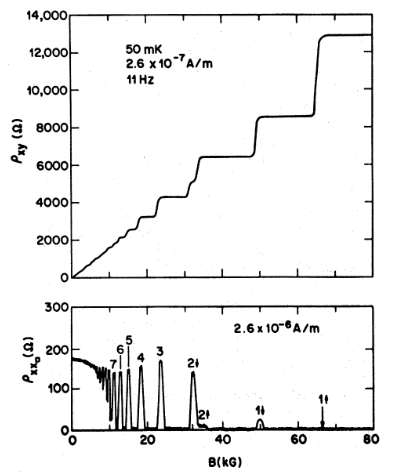
\includegraphics[height=5cm,width=5cm]{figs/future/IQHE_data_RHOxy_RHOxx}
	\caption[Example data of the Integer Quantum Hall Effect]{$\rho_{xy}$ as a function of magnetic field $B$ at low temperature ($T=50\unita{mK}$). Figure originally appeared in ref.~\cite{Paalanen_PhysRevB1982}.}
	\label{fig:IQHE_data}
\end{figure}
Fig.~\ref{fig:IQHE_data} demonstrates an example of the quantized nature of the transverse resistivity. The distance between each plateau (step height) is given by $h/e^2$ divided by an integer $i$. These steplike increases with plateaus in the magnetic field region where the longitudinal resistivity $\rho_{xx}$ vanished \cite{Klitzing_RevModPhys1986}. Thus, when $\rho_{xx} = 0$ then $\rho_{xy} = h/i e^2$ and is at a plateau. Note that the temperatures needed to observe the \acs{IQHE} ($\lesssim 4\unita{K}$) is a likely reason why it was not discovered until 1980. It is also important to note that the value of resistivity only depends on fundamental constants of physics and can be used as a primary resistance standard known as the von Klitzing constant, $R_{\mathrm{K}-90} = 25812.807\unita{\Omega}$ \cite{Klitzing_PhysRevLett1980,Aoki_PhysRevLett1986,Bliek_Met1988}. Observation of the \acs{IQHE} confirms the high-quality nature of the device in question as it is necessary to obtain high mobilities at very low temperatures. Furthermore, this would offer a more complete picture of the quantum structure of under the high-field limit and allow for the measurement of further quantum properties that reveal important information about the underlying structure of the device.%\\ \\ 

\section{Shubnikov-de Haas Oscillations}\label{sec:qm_oscillations}
There are several techniques and measurements that can determine the geometry of the Fermi surface, many of these are closely related to one another and are based on the same underlying mechanism. One such effect is the \acs{SdH} effect \cite{Shubnikov_Leiden1930}. The \acs{SdH} effect is an oscillatory dependence of the resistivity on the magnetic field, there it is related to the \ac{QHE} \cite{Soule_PhysRev1964}. This effect is produced by the oscillation of the density of states at the Fermi level which is caused by the quantization of electron energy levels in the presence of a magnetic field (see sec.~\ref{sec:IQHE}, Landau levels) \cite{Peierls_ZPhys1933,Landau_RoyalSoc1939}. The oscillations occur with a periodicity of $B^{-1}$ \cite{Shoenberg_Magnet1984}.\\ \\
\begin{figure}[ht]
	\centering
	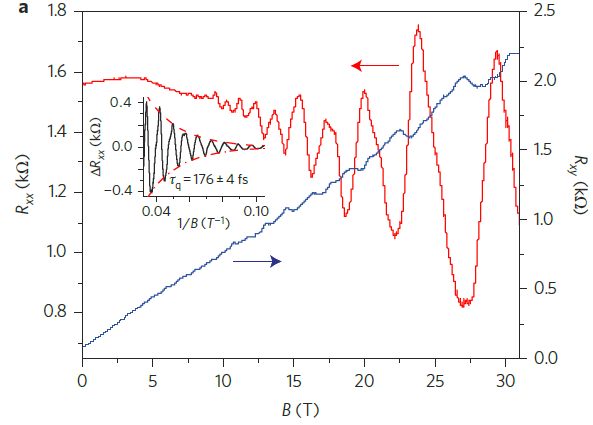
\includegraphics[height=6cm,width=8cm]{figs/future/mos2_SdH_oscillations}
	\caption[\ch{MoS2} quantum Hall effect and Shubnikov-de Haas oscillations]{Longitudinal resistance $R_{xx}$ (red curve) and Hall resistance $R_{xy}$ (blue curve) of an encapsulated \hbn \ac{CVD} monolayer \ch{MoS2} device as a function of magnetic field $B$ at $T=0.3\unita{K}$ with carrier density $n=9.7\times 10^{12}\unitb{cm}{-2}$. Inset: Oscillation amplitude (black curve) as a function of $B^{-1}$ with fitted plot for obtaining $\tau_q$. Figure appeared in ref \cite{Cui_NatureNano2015}.}
	\label{fig:mos2_SdH}
\end{figure}
\acs{SdH} oscillations can provide a wealth of information about the effective \acs{2DEG} (\acs{2DHG}). For example, one can extract the carrier lifetimes, effective cyclotron mass, information about the Fermi surface \cite{Li_NatureNano2015}. In order to observe the \acs{QHE} and therefore observe \acs{SdH} oscillations, high device mobility is required \cite{Das_Wiley1996,Tsukazak_Science2007}. Recently the Cui \emph{et al.} observed the first \acs{SdH} oscillations in \ch{MoS2}, Li \emph{et al.} and Gillgren \emph{et al.} observed this same effect in black phosphorus (and phosphorene) \cite{Cui_NatureNano2015,Li_NatureNano2015,Gillgren_2DMat2015}. Cui \emph{et al.} were able to determine geometry of the Fermi surface from the oscillation frequency and prove the two-dimensional nature of their system. Furthermore, from the analysis of the oscillation amplitude the cyclotron effective masses of both electrons and holes could be determined. From this method the carrier lifetime could also be determined, they reported lifetimes of $\tau = 0.11\unita{ps}$ and $\tau = 0.12\unita{ps}$ for holes and electrons, respectively \cite{Li_NatureNano2015,Shoenberg_Magnet1984}. Cui \emph{et al.} was able to provide insight about the quantum lifetimes and the underlying interactions between short-range and long-range scattering limits \cite{Cui_NatureNano2015}. Fig.~\ref{fig:mos2_SdH} shows the results from Cui \emph{et al.}. The red curve shows the longitudinal resistance $R_{xx}$, the blue curve shows the Hall resistance $R_{xy}$ both as a function of magnetic field $B$. The curve for $R_{xy}$ shows the plateaus for corresponding to the Landau levels. The inset of the curve also shows the \acs{SdH} oscillations as a function of $B^{-1}$, from this curve the quantum scattering lifetime of $\tau_q=0.18\unita{ps}$ in \acs{CVD} monolayer \ch{MoS2} is found by using a fit. The results provide promise that with the implementations of improvements in contact resistance reduction and further mobility enhancement that the world of \acp{TMD} is closer to the routine study of novel quantum physics in \td systems. 

\section{Performance Limits in \acp{TMD}}\label{sec:performance_limits}
The ultimate performance limit of \acp{TMD} is of interest, especially at room temperature as this is most relevant to device applications. 
%Again, one of the main obstacles that hinders from gaining definitive insight in this area is contact resistance. 
First principles calculations show mobility in monolayer \ch{MoS2} to be $\sim 320-410\cmvs$ at room temperature depending on initial parameters \cite{Li_PhysRevB2013,Kaasbjerg_PhysRevB2012}. Previously the experimental values reported differed by an order of magnitude compared to first principles calculations, however, the improvements made in the area of reducing contact resistance has improved mobility measurements \cite{Radisavljevic_NatureNano2011,Kappera_APLmat2014}. Experimentally, room temperature mobility measurements of both $p$ and $n$ type semiconductors still lag behind the theoretical calculations. For example, \ch{WSe2} room temperature mobilities have been reported as $\sim 200\cmvs$ with perfect subthreshold swings of $\sim 60\unita{mV}/\unita{dec}$, a $I_\mathrm{on}/I_\mathrm{off}$ of $> 10^6$ at room temperature (others have shown $I_\mathrm{on}/I_\mathrm{off}$ of $> 10^7$ in \ch{WSe2} and \ch{MoS2}), and high $I_\mathrm{on} \sim 300\unita{\mu A}/\unita{\mu m}$ \cite{Fang_NanoLett2012,Liu_NanoLett2013,Kappera_NatureMat2014,Das_NanoLett2014}. Undoped samples have shown to have room temperature mobility of an order of magnitude less than the doped counterparts \cite{Li_NanoLett2013,Das_NanoLett2014}. Note that these values are not the theoretical limits, but rather represent a current state of where measurements can achieve. To further improve the mobilities measured at room temperature a further understanding of scattering mechanisms is needed. At room temperature phonon scattering limits the mobility, the mobility can be enhanced by doping, however, this introduces impurities and can have an adverse effect on the mobility. Understanding the performance limit at room temperature in monolayers (and few layers) is key to applications in which several \acp{TMD} are already being implemented, such as \ac{TFT} and components of \acp{IC} like analog amplifiers, digital inverters, and memory transistors \cite{Bhimanapati_ACSnano2015,Akinwande_NatureComm2014,Lee_Small2012}.

\section{Conclusion}\label{sec:conclusion}
Overall, \acp{TMD} offer a wealth of opportunities in applications. In order to realize these proposed applications several challenges must be overcome, namely achieving low-resistance contacts and high mobility at room temperature. The approach of using degenerately doped contacts and \hbn encapsulated devices to lower the \acs{SBH} and promote increased mobility has shown potential. In addition, the increased mobility that the success of this method would allow one to study quantum transport properties which will reveal many fundamental properties, such as quantum scattering times and effective masses. 